\section{Design}
In the following section, the design of the project is presented, starting from the architecture-wise decisions and proceeding with the detailed design.

\subsection{Architectural Design}
As we have seen in the previous chapters, the project aims to develop a mechanism for the creation of distributed multi-agent systems using \textit{JaKtA}.
The team has decided to achieve this goal by providing an extension of the framework and its \textit{Domain Specific Language} that is as minimal as possible.
From an architectural point of view, the project is a standalone module, as shown in figure \ref{fig:architecture}:

\begin{figure}[ht!]
    \centering
    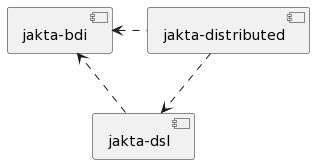
\includegraphics[width=0.8\textwidth]{figures/general-architecture.png}
    \caption{Architecture of the project}
    \label{fig:architecture}
\end{figure}

In particular, the developed module is composed of three main components, as shown in figure \ref{fig:detailed-architecture}:

\begin{figure}[ht!]
    \centering
    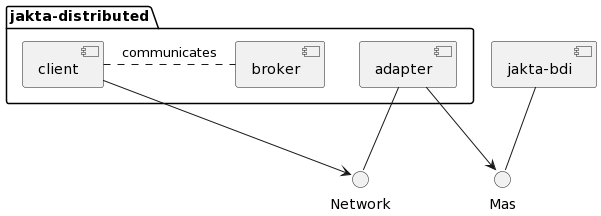
\includegraphics[width=0.8\textwidth]{figures/detailed-architecture.png}
    \caption{Detailed architecture of the project}
    \label{fig:detailed-architecture}
\end{figure}

Of the modules represented in figure \ref{fig:detailed-architecture}, the \textit{Adapter} module is the one that defines and contains all the concepts to be implemented to achieve the project goal,
while the \textit{Client} and \textit{Broker} modules provide a first implementation of the communication logic between distributed multi-agent systems.\\

As previously mentioned, the project also presents an extension of the JaKtA \textit{Domain Specific Language}, whose structure is represented in figure \ref{fig:dsl-architecture}.

\begin{figure}[ht!]
    \centering
    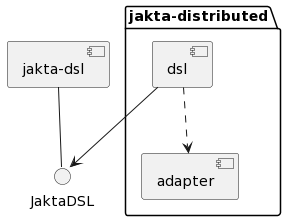
\includegraphics[width=0.8\textwidth]{figures/dsl-architecture.png}
    \caption{Domain Specific Language architecture}
    \label{fig:dsl-architecture}
\end{figure}

\subsubsection{Network Architecture}
The component diagram shown in Figure \ref{fig:network-architecture} provides an overview of the network architecture.

The \textit{Broker} exposes four interfaces: the \textit{/subscribe/{topic}} and \textit{/publish/{topic}} interfaces allow respectively the subscription and publication on specific topics, while the topics interface allows to retrieve the list of available topics. Furthermore, the \textit{/subscribe-all/\{except...\}} interface offers the possibility to subscribe to all topics except those specified. The \textit{MAS}, on the other hand, connects to the \textit{Broker} through these interfaces, using them to subscribe, publish and obtain information from the other \textit{MAS}. This setup allows the management of distributed communications, with the \textit{Broker} acting as a central hub to facilitate the subscription, publication and management of topics within the system.

\begin{figure}[ht!]
    \centering
    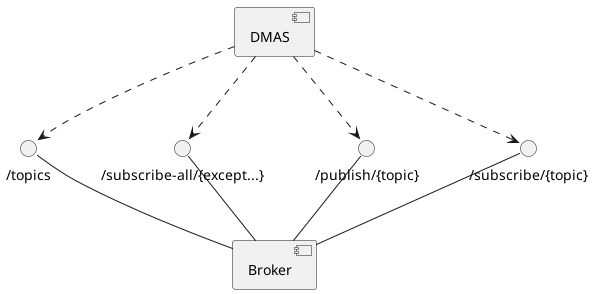
\includegraphics[width=0.8\textwidth]{figures/network-architecture.png}
    \caption{Network architecture}
    \label{fig:network-architecture}
\end{figure}

\subsection{Detailed Design}
When designing an extension of the framework that allows communication between distributed multi-agent systems, it is important to establish what is shared between these systems.
To this end, there are several possibilities to consider:

%\begin{itemize}
%    \item Condividere l'\textit{Environment}: in questo caso, gli agenti di ogni sistema multi-agente operano nello stesso \textit{Environment}. Questa soluzione è stata ritenuta complessa e rischiosa da implementare,
%          poiché l'\textit{Environment} è una struttura dati complessa e cruciale per il funzionamento del sistema multi-agente, e la sua condivisione tra più sistemi richiederebbe una gestione molto robusta della consistenza dei dati tra i vari sistemi;
%    \item Condividere gli agenti: in questo caso, sistemi multi-agente diversi possono condividere agenti. Questa soluzione è un sottoinsieme della precedente, ma presenta gli stessi problemi;
%    \item Condividere i messaggi tra gli agenti: in questo caso, sistemi multi-agente diversi possiedono \textit{Environment} ed agenti diversi, ma gli agenti di un sistema possono inviare messaggi agli agenti di un altro sistema.
%\end{itemize}
%
%Il team ha ritenuto l'ultima soluzione la più semplice ed efficace da implementare, in quanto la condivisione di un messaggio non presenta le stesse criticità dell'implementazione di strutture dati condivise. Inoltre si ritiene che questa soluzione offra comunque grande flessibilità e possibilità di realizzare comportamenti complessi tra i vari sistemi multi-agente.

\paragraph{Sharing the Environment}: in this case, the agents of each multi-agent system operate in the "same" \textit{Environment}.
This means that any modification that may happen on the environment is known by each distributed Mas, for example:
\begin{itemize}
    \item agent creation;
    \item agent deletion;
    \item actions;
    \item messages exchanged between agents;
    \item any data added or removed from the environment.
\end{itemize}

This solution allows for easy programming of the distributed system, since the environment and the agents it contains are the same for each distributed Mas, making it possible for the programmer to write the program as if it were a single Mas.
However, this solution presents some technical problems:
\begin{enumerate}
    \item The environment is a complex data structure, and its sharing between multiple systems requires very robust management of data consistency between the various systems;
    \item If the environment is shared, this means that any sort of modification is propagated to the network, to keep the environments in each distributed Mas consistent. This
          can lead to a lot of network traffic, putting pressure on the broker services;
    \item This solution does not allow for the creation of multiple environments, which could be useful in some cases.
\end{enumerate}

\paragraph{Sharing messages}: in this case, different multi-agent systems have different environments and agents, but the agents of a system can send messages to the agents of another system, both in a one-to-one fashion and in a one-to-many fashion.
This solution embodies the idea of "do not communicate by sharing memory; instead, share memory by communicating" and is a technically easier solution to implement than the previous one, since it does not require a robust management of data consistency between the various systems.
Also, it could be more flexible regarding programmer needs since it allows for the creation of multiple environments, and the programmer can decide which messages to share between the various systems.

However, this solution is somewhat limited in some respects:
\begin{itemize}
    \item The only way to share data between the various systems is through communication, so the programmer needs to instruct the agents to send messages to agents in the other systems;
    \item Since the environments are not shared, the programmer needs to take care of the consistency of the data between the various systems;
    \item Again, not sharing the environments means that the programmer needs to design multiple distributed Mas', as opposed to the previous solution.
\end{itemize}

In summary, this solution removes some complexity from the distributed infrastructure design but puts some on the programmer's shoulders.
Regardless, after some discussion, taking into account the project's scope and technical difficulties, the team decided to implement the second solution, valuing its simplicity and flexibility.\\

So the proposed solution consists of the implementation of an alternative version of the \texttt{Mas} interface, called \texttt{Dmas}, to be used in distributed contexts.
This extension should behave like a \texttt{Mas}, but in addition, should be able to communicate with other \texttt{Dmas} through the network.
The communication model chosen is the \textit{publish-subscribe} model, which allows for a simple and effective communication between the various \texttt{Dmas}.
In this context, every agent is associated with a unique \textit{topic}, so
to enable an effective communication, it is necessary for two agents to know each other's \textit{topic} in advance.
This association enables targeted and organized communication, aiming for agents to focus solely on information relevant to their scope,
thereby facilitating the coordination of activities in the whole system.

\subsubsection{Adapter}
This module defines the concepts of:

\begin{itemize}
    \item \textbf{Dmas}: represents a distributed multi-agent system, i.e. a system that can communicate with other \texttt{Dmas} through the network;
    \item \textbf{Network}: encapsulates the logic for the communication between \texttt{Dmas};
    \item \textbf{RemoteService}: represents a remote agent, i.e. an agent that belongs to a \texttt{Dmas} different from the current one, but reachable through the network.
\end{itemize}

The relationships between these concepts are exemplified by the class diagram in figure \ref{fig:class-dmas}.

\begin{figure}[ht!]
    \centering
    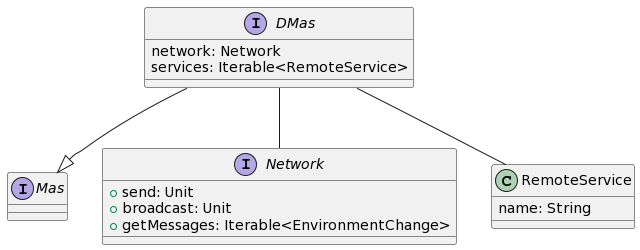
\includegraphics[width=0.8\textwidth]{figures/class-dmas.png}
    \caption{Adapter class diagram}
    \label{fig:class-dmas}
\end{figure}

\subsubsection{Broker}

In the design and implementation of our system, a dedicated broker has been introduced to cater to specific requirements and unique behavioral patterns. This decision was driven by the need for nuanced control over message publication and subscriptions, differentiating our broker from conventional MQTT or AMQT brokers. Several motivations underpin this choice:

Our broker deviates from the conventional MQTT or AMQT model by enforcing a distinct behavior: for a given topic, only a single client can publish messages at any given time. This ensures a controlled and orderly flow of information, avoiding conflicts that may arise when multiple clients attempt simultaneous publications on the same channel.

While adhering to the exclusive publishing behavior for most topics, exceptions are made for specific topics, such as the "broadcast" topic. Topics falling under this category do not follow the stringent single-client publishing rule, allowing for broader dissemination of information.

A pivotal aspect of our dedicated broker lies in the introduction of specialized error-handling mechanisms. Notably, in the event of a publisher disconnecting, the broker takes proactive measures to notify the disconnection to the subscribers. This tailored approach to error management ensures that clients are promptly informed of disruptions, facilitating responsive and effective handling of disconnection scenarios.

The \textit{broker}'s class diagram (Figure \ref{fig:broker-class-diagram}) presents a modular and organized structure.
Inside the \texttt{model} package, two key interfaces are defined: \texttt{Cache<T>} for registering, releasing and reading data associated with a \textit{topic}, and \texttt{SubscriptionManager<T>} for managing the subscription, addition and removal of \textit{publishers} and \textit{subscribers}, as well as obtaining the available \textit{topics} and the \textit{subscribers} associated with a \textit{topic}.
The \texttt{plugins} package includes the \texttt{Routing} and \texttt{Websockets} classes, which are used to define the \textit{Web APIs}.

\begin{figure}[ht!]
    \centering
    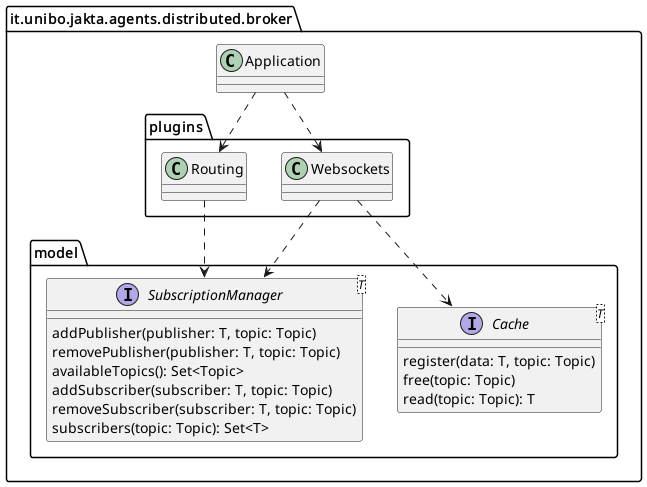
\includegraphics[width=0.8\textwidth]{figures/broker-class-diagram.png}
    \caption{Broker class diagram}
    \label{fig:broker-class-diagram}
\end{figure}

\subsection{Behavior}
The behavior of the various components of the system can be described through the following steps.

\subsubsection{System Initialization}

\begin{enumerate}
    \item \textit{Network} initialization;
    \item connection between Network and \textit{Broker};
    \item definition of the \textit{RemoteService}s of interest;
    \item \textit{Dmas} creation;
    \item for each RemoteService, the Dmas subscribes to the according \textit{topic};
    \item \textit{ExecutionStrategy} dispatching;
\end{enumerate}

These activities are showcased in the figure \ref{fig:initialization}.

\begin{figure}[ht!]
    \centering
    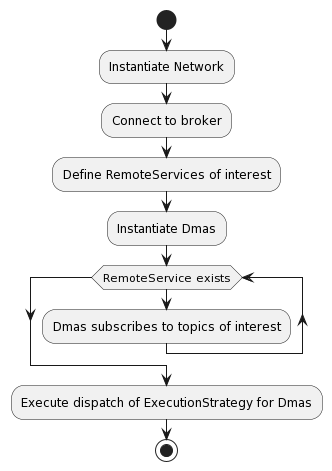
\includegraphics[width=0.8\textwidth]{figures/activity-dmas.png}
    \caption{System initialization}
    \label{fig:initialization}
\end{figure}

\subsubsection{Dmas execution cycle}

\begin{enumerate}
    \item the \texttt{Dmas} collects all the external events received from the \texttt{Network},
          i.e. the messages published by the \texttt{RemoteService}s to which it has subscribed and the eventual disconnection notifications of a \texttt{RemoteService},
          in the form of \texttt{EnvironmentChange};
    \item external events are concatenated to the queue of internal EnvironmentChanges of the Dmas;
    \item one by one, the \texttt{EnvironmentChange}s are processed by the \texttt{Dmas}. In case the event consists of sending a message to a \texttt{RemoteService} or a \textit{broadcast}, the message is sent to the \texttt{Network}, which will forward it to the \textit{broker};
\end{enumerate}

These activities are showcased in the figure \ref{fig:execution}.

\begin{figure}[ht]
    \centering
    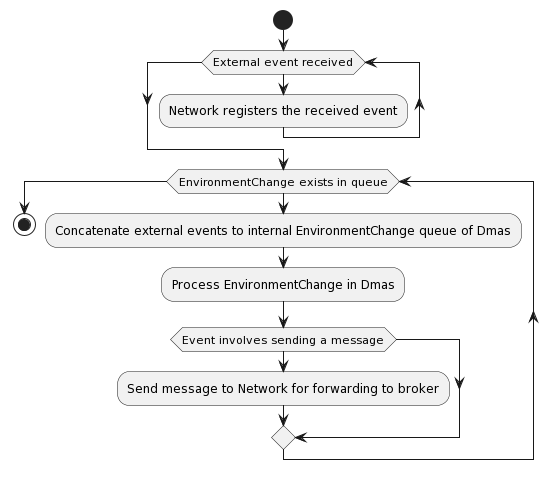
\includegraphics[width=0.8\textwidth]{figures/activity-applychanges.png}
    \caption{Dmas execution cycle}
    \label{fig:execution}
\end{figure}

\subsection{Interaction}
The interaction model between the various \texttt{Dmas} connected to the network is of the \textit{publish-subscribe} type: each \texttt{Dmas}, which assumes the role of \textit{client}, can subscribe to one or more \textit{topics}, and can publish messages on one or more \textit{topics}.
Published messages are received by all \textit{clients} that have subscribed to the \textit{topic} to which the message was published.
It is relevant to note that agents know each other's \textit{topic}.


The \textit{broker}, which assumes the role of server, is responsible for managing the communication between the \textit{clients}, in particular, it is responsible for:
\begin{itemize}
    \item receiving the messages published by the \textit{clients};
    \item sending the messages to the \textit{clients} subscribed to the corresponding \textit{topics};
    \item managing the connections and disconnections of the \textit{clients}.
    \item managing the subscription of the \textit{clients} to the various \textit{topics}.
\end{itemize}

\begin{figure}[ht!]
    \centering
    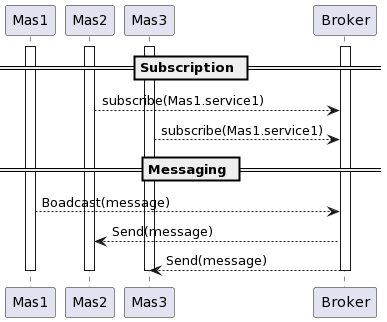
\includegraphics[width=0.8\textwidth]{figures/interaction-broadcast.png}
    \caption{Interaction between DMas, \textit{client} and \textit{broker} in case of \textit{broadcast}}
    \label{fig:interaction-broadcast}
\end{figure}

\begin{figure}[ht!]
    \centering
    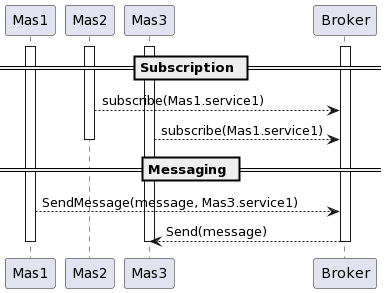
\includegraphics[width=0.8\textwidth]{figures/interaction-sendmessage.png}
    \caption{Interaction between DMas, \textit{client} and \textit{broker} in case of sending a message to a single recipient}
    \label{fig:interaction-sendmessage}
\end{figure}

The behavior of \textit{client} and \textit{broker} in situations of \textit{broadcast} and sending of messages with a single recipient is illustrated in figures \ref{fig:interaction-broadcast} and \ref{fig:interaction-sendmessage}.

\subsubsection{Publishers with the same name} \label{sec:publishers-same-name}

From the point of view of the Dmas, the interaction in the case of a \textit{sendmessage} is comprised of the following steps:
\begin{itemize}
    \item when an agent in the Dmas sends a message to an agent outside of it, the Dmas sends a message to the \textit{broker} via his \textit{Client} containing the message to be sent and the \textit{topic} of the recipient;
    \item the broker checks whether or not the publisher's name is valid;
    \item if the check ended with a success, the message is forwarded, otherwise the broker closes the connection with the client;
\end{itemize}

this interaction is illustrated in figure \ref{fig:interaction-sendmessage-pov}.

\begin{figure}[ht!]
    \centering
    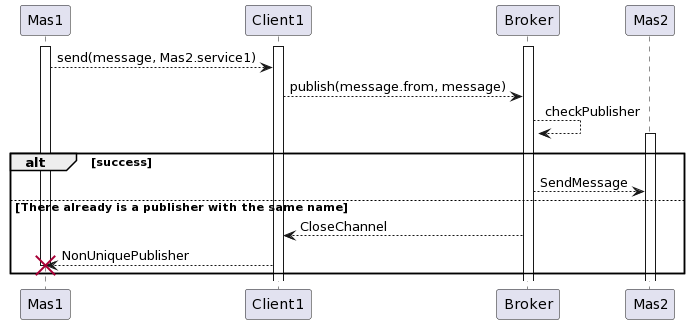
\includegraphics[width=0.8\textwidth]{figures/interaction-sendmessage-pov.png}
    \caption{Sequence diagram of the interaction between \texttt{Dmas}, his \textit{client} and \textit{broker} in case of sending a message to a single recipient}
    \label{fig:interaction-sendmessage-pov}
\end{figure}


\subsubsection{Disconnection management}
Since the system is distributed, it is important to assume that disconnections of any participant in the system may occur, be it a \texttt{Dmas} or the \textit{broker}.
The general strategy of the system is to create, in the event of a disconnection, an \texttt{EnvironmentChange} of type \texttt{SendMessage} for each agent of the \texttt{Dmas} subscribed to the
disconnected participant, so that they can be informed of the disconnection and act accordingly. It is important to note that this strategy leaves the task of managing failures to the programmer of the agents of the \texttt{Dmas}.

\begin{figure}[ht!]
    \centering
    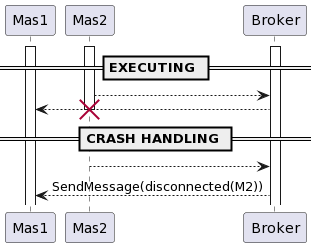
\includegraphics[width=0.8\textwidth]{figures/sequence-client-crash.png}
    \caption{Interaction between \texttt{Dmas}, \textit{client} and \textit{broker} in case of \textit{client} disconnection
        \label[type]{fig:interaction-disconnect}}
\end{figure}

\begin{figure}[ht!]
    \centering
    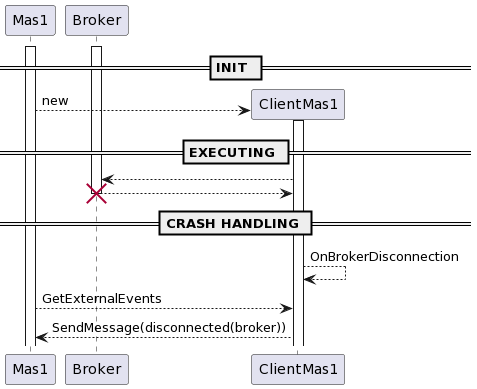
\includegraphics[width=0.8\textwidth]{figures/sequence-broker-crash.png}
    \caption{Interaction between \texttt{Dmas}, \textit{client} and \textit{broker} in case of \textit{broker} disconnection}
    \label{fig:interaction-disconnect-broker}
\end{figure}

Figures \ref{fig:interaction-disconnect} and \ref{fig:interaction-disconnect-broker} show how the system manages the disconnections from \texttt{Dmas} and \textit{broker}.
